\documentclass{article}
\usepackage[utf8]{inputenc}
\usepackage{graphicx}
\usepackage{natbib}

\begin{document}
\title{Relatório Técnico 1}
\author{Rodrigo R. G. e Souza}
\maketitle

\section{Redes de Dependências entre Componentes}

Sistemas de \textit{software} precisam ser modificados constamente. Dependências excessivas entre os componentes de um sistema podem tornar as modificações mais custosas, uma vez que dificultam a compreensão dos componentes isoladamente. Por essa razão o estudo de redes formadas por dependências entre componentes de \textit{software} pode fornecer pistas sobre a atividade de desenvolvimento de \textit{software} em geral.
% interação entre componentes

Neste trabalho consideramos como componentes as entidades de código-fonte, tais como classes, métodos e atributos (no caso de linguagens orientadas objetos), ou procedimentos, funções e tipos abstratos de dados (no caso de linguagens procedimentais). Dizemos que um componente depende de outro quando o funcionamento do primeiro está condicionado à presença do segundo. Dependências podem se originar de diversos tipos de interação, como uma chamada a uma função ou a leitura de um atributo. Dependências são essencialmente assimétricas: o fato de um componente A depender de um componente B não implica que B depende de A.

% Um relacionamento de dependência indica que as alterações em um elemento do modelo (fornecedor ou independente) podem causar alterações em um outro elemento do modelo (cliente ou dependente). http://publib.boulder.ibm.com/infocenter/rsmhelp/v7r5m0/index.jsp?topic=/com.ibm.xtools.modeler.doc/topics/rreltyp.html

\subsection{Extração}

A rede de dependências entre componentes de um sistema pode ser extraída automaticamente por um programa construído para este fim, denominado extrator de dependências. As principais abordagens de extração de dependências são a análise dinâmica e a análise estática. 

A análise dinâmica envolve a instrumentação do sistema para coletar dados de sua execução, e por isso exige que o programa esteja corretamente instalado e configurado. Para que seja efetiva, é preciso que o programa sob análise seja executado com as mais diversas entradas a fim de 

%For dynamic program analysis to be effective, the target program must be executed with sufficient test inputs to produce interesting behavior
%Also, care must be taken to minimize the effect that instrumentation has on the execution

%e depende da execução de diversos cenários de uso. 

A análise estática é realizada sobre o código-fonte ou o código objeto do sistema, dispensando sua execução.

Nenhuma técnica automática é capaz de determinar corretamente, em todos os casos, se existe uma dependência entre dois componentes, pois esse é um problema indecidível \cite{Landi1992} --- basta considerar o uso de ponteiros em linguagens como C++, ou a transferências de dados através de arquivos. Assim, redes de dependências extraídas automaticamente devem ser consideradas apenas aproximações das redes de dependências reais.

\subsection{Simplificação e Detalhamento}

A depender do tipo de análise que se deseja realizar sobre uma rede de dependências, pode ser conveniente filtrar ou contrair componentes, ou mesmo tratar dependências como relacionamentos simétricos. A filtragem consiste em remover componentes ou dependências consideradas desnecessárias para a análise. A contração pode ser feita quando há uma relação de composição entre os componentes, como no caso de classes (que são compostas de atributos e métodos). Nesse caso uma classe e todos os atributos e métodos que a compõem podem ser representados como um só componente. % e aí surgem dependências implícitas: A.m1 depende de B.m2 implica A depende (implicitamente) de B.
% http://depfind.sourceforge.net/Manual.html#Dependencies

Há análises que, por outro lado, requerem informações mais detalhadas. Pode ser necessário considerar não apenas a existência de dependências, mas também identificar quais são os tipos de interações que ocorrem entre dois componentes e com que frequência essas interações ocorrem.

\section{Redes Complexas}

A teoria das redes complexas estuda propriedades gerais de diversos tipos de redes com o uso de ferramentas estatísticas. Estudos realizados na última década revelaram similaridades entre diversas redes, sejam elas tecnológicas, como a Web e a rede de distribuição de energia elétrica dos Estados Unidos, biológicas, como a cadeias alimentares e ligações entre proteínas, ou sociais, como as relações de amizade entre alunos de uma escola.

\subsection{Distribuição de Graus}

% histograma de frequências do número de ligações por vértice
% distribuição de probabilidades
% expoente gamma entre 2 e 3.
Barabási e Albert (\citeyear{Barabasi1999}) analisaram uma amostra da \textit{World Wide Web}, modelada como um grafo não-orientado no qual os vértices representam páginas e as arestas representam \textit{links} entre duas páginas. Eles perceberam que a probabilidade de um vértice escolhido ao acaso ter grau $k$ (isto é, estar ligado a $k$ arestas) seguia uma lei de potência: $p(k) \sim k^{-\gamma}$. Dizemos, nesse caso, que a rede possui uma distribuição de graus livre de escala, ou simplemente que a rede é livre de escala. Desde então esse tipo de distribuição foi encontrado em diversas redes, incluindo redes de dependências entre componentes de programas de computador \cite{Valverde2003}.

\begin{figure} \label{fig:leidepotencia}
\centering
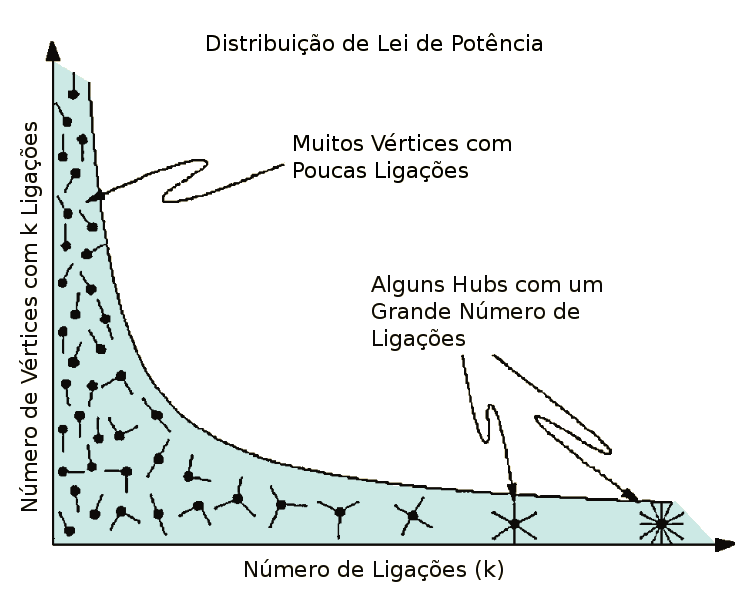
\includegraphics[width=0.5\textwidth]{leidepotencia}
\caption{Distribuição de graus como lei de potência. Adaptado de \cite{Barabasi2007}.}
\end{figure}

Esse resultado foi considerado surpreendente, pois contradiz a hipótese de que redes reais obedecem ao modelo de Erdős-Rényi (\citeyear{Erdos1959}), também chamado de modelo de rede aleatória. Nesse modelo, a probabilidade de um par de vértices ser ligado por uma aresta é constante e igual a $p$. Demonstra-se que a distribuição dos graus de redes geradas por esse modelo é bem aproximada pela distribuição de Poisson.

Uma característica das redes livres de escala é a presença de vértices cujo grau é muito maior do que a média (informalmente chamados de \textit{hubs}). No caso de redes de Erdős-Rényi a probabilidade de existir um vértice com um determinado grau $k$ cai exponencialmente à medida que $k$ se afasta do valor médio e, por essa razão, nessas redes os \textit{hubs} são altamente improváveis.

Barabási e Albert propuseram um modelo para explicar a formação das redes com distribuição de graus livre de escala, formado por dois mecanismos: crescimento contínuo e ligação preferencial \cite{Albert2002}. O modelo propõe que as redes crescem um vértice por vez e cada novo vértice se liga a um número fixo de vértices antigos, dando preferência aos vértices com maior grau (mais formalmente, a probabilidade de um vértice receber uma aresta é proporcional ao seu grau). Hoje sabe-se que redes livres de escala também podem ser geradas por outros modelos \cite{Albert2000,Kumar2000,Aiello2000b,Dorogovtsev2002,Bollobas2003,Deo2005}.

% Cada vértice em um grafo é caracterizado por um grau, k, que representa a quantidade de arestas ligadas a ele. No caso de grafos orientados, existe a distinção entre grau de saída e grau de entrada, que representam a quantidade de arcos que saem ou entram, respectivamente, do vértice.

\subsubsection{Efeito Mundo Pequeno}

A distância entre dois vértices de uma rede é o número de arestas do menor caminho que conecta os vértices. Diz-se que uma rede apresenta o efeito mundo pequeno quando a distância entre dois vértices é, em média, pequena, mesmo quando a rede é grande. Mais formalmente, a distância média entre vértices é proporcional ao logaritmo do número de vértices \cite{Watts1998}. Esse efeito foi detectado em diversas redes reais.

%Demonstra-se que tanto os grafos gerados pelo modelo de Erdős-Rényi quanto aqueles gerados pelo modelo de Barabási-Albert possuem essa propriedade.

% Nesse modelo os vértices são dispostos em uma circunferência e então cada vértice se conecta a um número fixo de vértices mais próximos. O grafo resultante é regular, isto é, todos os seus vértices possuem o mesmo grau. A seguir são criadas arestas entre pares de vértices escolhidos aleatoriamente. Essas arestas criam atalhos na rede e fazem com que a rede tenha a propriedade de mundo pequeno. // Rewire

\subsubsection{Coeficiente de agrupamento}

Os vizinhos de um vértice são todos os vértices com os quais ele compartilha uma aresta. O coeficiente de agrupamento de um vértice, $C_i$, é a fração de todos os possíveis pares de vizinhos do vértice que estão ligados por uma aresta, e é dado pela seguinte expressão:

\[  C_i = \frac{2x}{k_i(k_i - 1)} \]

onde $x$ é o número de pares de vizinhos do vértice $i$ que estão ligados por uma aresta e $k_i$ é o grau do vértice $i$ \cite{Watts1998}. Por definição, $C_i = 0$ quando $k_i < 2$. Define-se o coeficiente de agrupamento de um grafo, $C$, como a média aritmética dos coeficientes de agrupamento dos seus vértices. Demonstra-se que o coeficiente de agrupamento de uma rede aleatória de Erdős-Rényi é igual a $\langle k \rangle / n$ (onde $\langle k \rangle$ é o grau médio). Muitas redes complexas possuem um coeficiente de agrupamento alto, isto é, muito maior do que o coeficiente das redes aleatórias.

Outra característica observada em algumas redes é que o coeficiente de agrupamento de um vértice é inversamente proporcional ao grau do vértice, ou seja, $C(k) \sim k^-1$. Segundo Ravasz e Barabási \cite{Ravasz2003}, isso indica a existência de uma organização hierárquica na rede.

\subsubsection{Motivos}

Motivos são padrões de vértices e arestas que ocorrem com frequência em uma rede \cite{Milo2002}. Estudos recentes encontraram em redes de dependências entre componentes motivos presentes em redes de neurônios e em circuitos eletrônicos \cite{Valverde2005,Ma2008}. Especula-se que a formação de motivos seja resultado de restrições de custo e otimização impostas à evolução de sistemas de \textit{software}.

% \subsubsection{Assortatividade, mixing}

\section{Redes de Dependências entre Componentes como Redes Complexas}

Estudos recentes têm aplicado a teoria das redes complexas em redes de dependências entre componentes de \textit{software}. Valverde e Solé \cite{Valverde2003} detectaram distribuições de graus livres de escala e alto coeficiente de agrupamento em redes não-orientadas formadas por relações de agregação de tipos em diagramas UML, programas em C e programas em C++. Myers \cite{Myers2003} analisou redes de chamadas de função em programas em C e redes de agregação e herança em programas em C++, modeladas como grafos orientados. Em ambos os casos ele identificou organização hierárquica através da distribuição do coeficiente de agrupamento, $C(k) \sim k^{-1}$. O estudo revelou uma correlação negativa entre o grau de entrada e o grau de saída de um vértice. Leis de potência foram encontradas em trechos das distribuições de graus de entrada e das distribuições de graus de saída.

Distribuições de graus livres de escala também foram encontradas em programas escritos em Smalltalk \cite{Marchesi2004,Concas2007} e em Java \cite{Hyland-Wood2006,Baxter2006,Ichii2008}, em dependências entre pacotes de \textit{software} \cite{Labelle2004}, em chamadas de sistema, em dependências entre bibliotecas dinâmicas \cite{Louridas2008} e até mesmo em referências entre objetos em tempo de execução \cite{Potanin2005}.

É difícil comparar as pesquisas porque nem sempre elas deixam explícito quais tipos de interação foram considerados para a construção das redes. Além disso, alguns trabalhos usam ferramentas estatísticas inadequadas para leis de potência (veja a seção \ref{sec:estatistica}).

%Nem todos os trabalhos usam a Estatística rigorosamente. Lognormal, double pareto, power law, stretched exponential, power law with exponential cutoff... Alguns usam o coeeficiente de determinação ($R^2$), que não se aplica a leis de potência, ou o método dos mínimos quadrados sobre o logaritmo dos dados.

\section{Apêndice: Tratamento Estatístico de Leis de Potência} \label{sec:estatistica}

% Assimétrica, heterogênea, cauda pesada
% cabeça, cauda: região extrema da distribuição 
% cauda pesada
% lei de potência = distribuição zeta
% ccdf

              The populations of cities, the intensities of earthquakes, and the sizes of
power outages, for example, are all thought to have power-law distributions. Quan-
tities such as these are not well characterized by their typical or average values.

    In practice, few empirical phenomena obey power laws for all values of x. More
often the power law applies only for values greater than some minimum xmin . In such
cases we say that the tail of the distribution follows a power law.


// Talvez aqui fazer algo didático, como no livro The Black Swan

. Unfortunately, the empirical detection and characterization of power laws is made difficult by the large fluctuations that occur in the tail of the distribution. In particular, standard methods such as least-squares fitting are known to produce systematically biased estimates of parameters for power-law distributions and should not be used in most circumstances. Here we describe statistical techniques for making accurate parameter estimates for power-law data, based on maximum likelihood methods and the Kolmogorov-Smirnov statistic. We also show how to tell whether the data follow a power-law distribution at all, defining quantitative measures that indicate when the power law is a reasonable fit to the data and when it is not. We demonstrate these methods by applying them to twenty-four real-world data sets from a range of different disciplines. Each of the data sets has been conjectured previously to follow a power-law distribution. In some cases we find these conjectures to be consistent with the data while in others the power law is ruled out.

Propriedades estatísticas da lei de potência. A Figura 1(a) mostra o gráfico de uma lei de potência. Intuitivamente, percebe-se que a grande maioria dos vértices possui um grau pequeno, mas existem vértices cujo grau está muito acima do grau médio. Trata-se de uma curva assimétrica positiva, pois a média é maior do que a mediana. A probabilidade de um elemento de grau alto é pequena mas não desprezível, e isso contribui para elevar a média. Como a distribuição é muito heterogênea, a média não é um valor muito representantivo da distribuição. A lei de potência, quando plotada em escala log-log, se apresenta sob a forma de uma reta. Dificilmente dados obtidos experimentalmente formam uma reta em toda sua extensão. Portanto muitas vezes quando se afirma que uma distribuição é livre de escala, o que se quer dizer é que parte da distribuição é bem aproximada por uma reta na escala log-log.

Tratamento estatístico de leis de potência:  \cite{Newman2005} - Power laws, Pareto distributions and Zipf's law   //   Clauset et al - Power-law distributions in empirical data \cite{Clauset2007}

histograma. problema com a escolha do tamanho do bin. histograma com exponential bins
distribuição cumulativa complementar (survival)
maximum likelihood estimation para estimar expoente. -- máxima verossimilhança
goodness-of-fit para estimar região de scaling.
não usar: regressão linear (método dos mínimos quadrados), coeficiente de determinação ($R^2$)


%%%%%%%%%%%%%%%%%%%%%%%%%%%%%%%%%%%%%%%%%%%%%%%%%%%%%%%%%%%%%%%%%%%%%%%%%%%%%%%%%%%%%%%%%%%%%%%
%%%%%%%%%%%%%%%%%%%%%%%%%%%%%%%%%%%%%%%%%%%%%%%%%%%%%%%%%%%%%%%%%%%%%%%%%%%%%%%%%%%%%%%%%%%%%%%
%%%%%%%%%%%%%%%%%%%%%%%%%%%%%%%%%%%%%%%%%%%%%%%%%%%%%%%%%%%%%%%%%%%%%%%%%%%%%%%%%%%%%%%%%%%%%%%
%%%%%%%%%%%%%%%%%%%%%%%%%%%%%%%%%%%%%%%%%%%%%%%%%%%%%%%%%%%%%%%%%%%%%%%%%%%%%%%%%%%%%%%%%%%%%%%

% Modelos: Bollobas, Deo and Cami

%%%%%%%%%%%%%%%%%%%%%%%%%%%%%%%%%%%%%%%%%%%%%%%%%%%%%%%%%%%%%%%%%%%%%%%%%%%%%%%%%%%%%%%%%%%%%%%
%%%%%%%%%%%%%%%%%%%%%%%%%%%%%%%%%%%%%%%%%%%%%%%%%%%%%%%%%%%%%%%%%%%%%%%%%%%%%%%%%%%%%%%%%%%%%%%
%%%%%%%%%%%%%%%%%%%%%%%%%%%%%%%%%%%%%%%%%%%%%%%%%%%%%%%%%%%%%%%%%%%%%%%%%%%%%%%%%%%%%%%%%%%%%%%


\section{Recuperação de Arquitetura}

\subsection{Arquitetura: Componentes e Conectores}

Componentes e conectores.
Visões. Processos, módulos.

\subsection{Técnicas de Recuperação de Arquitetura}


Análise dinâmica, análise estática. Padrões de nomes (Anquetil). Padrões estrutrais (LIMBO). Análise de clustering (Maqbool)



Sobre clustering. Referência: Introduction to Data Mining, capítulo 8

\subsubsection{Detecção de Comunidades}

= análise de clustering (graph clustering, network clustering), = recuperação de arquitetura modular (módulos de atribuição de trabalho).

Clauset, Newman, Moore - Finding community structure in very large networks \cite{Clauset2004}

Gulbahce2008 - "The art of community detection" \cite{Gulbahce2008}: Currently the state of the art is to design an artificial network with the structural properties that one wants to detect (e.g. group strucutre) and then show that the algorithm being tested is able to detect such structures. 

definição de cluster: A number of similar things collected together or lying contiguous; a group;

A community is
a densely connected subset of nodes that is only sparsely
linked to the remaining network. (Gulbahce)

Communities in a citation network might represent
related papers on a single topic;

Community can be considered as a summary of
the whole network thus easy to visualize and
understand.

relação funcional, módulos de funcionalidade


Modelo de Girvan-Newman - Newman - Fast algorithm for detecting community structure in networks \cite{Newman2004b} e, mais antigo, Newman, Girvan - Finding and evaluating community structure in networks \cite{Newman2004a}

Paper: Benchmark for community detection \cite{Lancichinetti2008}


\subsection{Tipos de Decomposições}

Referência: Introduction to Data Mining, capítulo 8 \cite{Tan2005}

Hierárquica vs partitiva.
Exclusive vs overlapping vs fuzzy.
Completa vs. parcial.

\subsection{Algoritmos}

Bunch. LIMBO. MCL etc. (a escolher)

\subsection{Avaliação de Decomposições}

Avaliação não-supervisionada: NED, estabilidade.
Avaliação supervisionada: authoritativeness.

Avaliações relativas (comparar dois algoritmos)

\subsection{Comparação entre Decomposições}

Precision-recall.
MoJo.
EdgeMoJo.
etc.

\bibliographystyle{apalike}
\bibliography{complex-networks,rodrigo-mestrado}

\end{document}
